%!TEX root = ../thesis.tex

%%%%%%%%%%%%%%%%%%%%%%
%    CMS detector    %
%%%%%%%%%%%%%%%%%%%%%%
\message{^^J ^^J DETECTOR ^^J ^^J} % print to log
\newchap{The CMS Experiment} \label{sec:dectector}

This chapter will discuss the experimental setup.

%!TEX root = ../thesis.tex

% FIGURE: accelerator
\begin{figure*}[b!]
  %\vspace{-2mm}
  \centering
  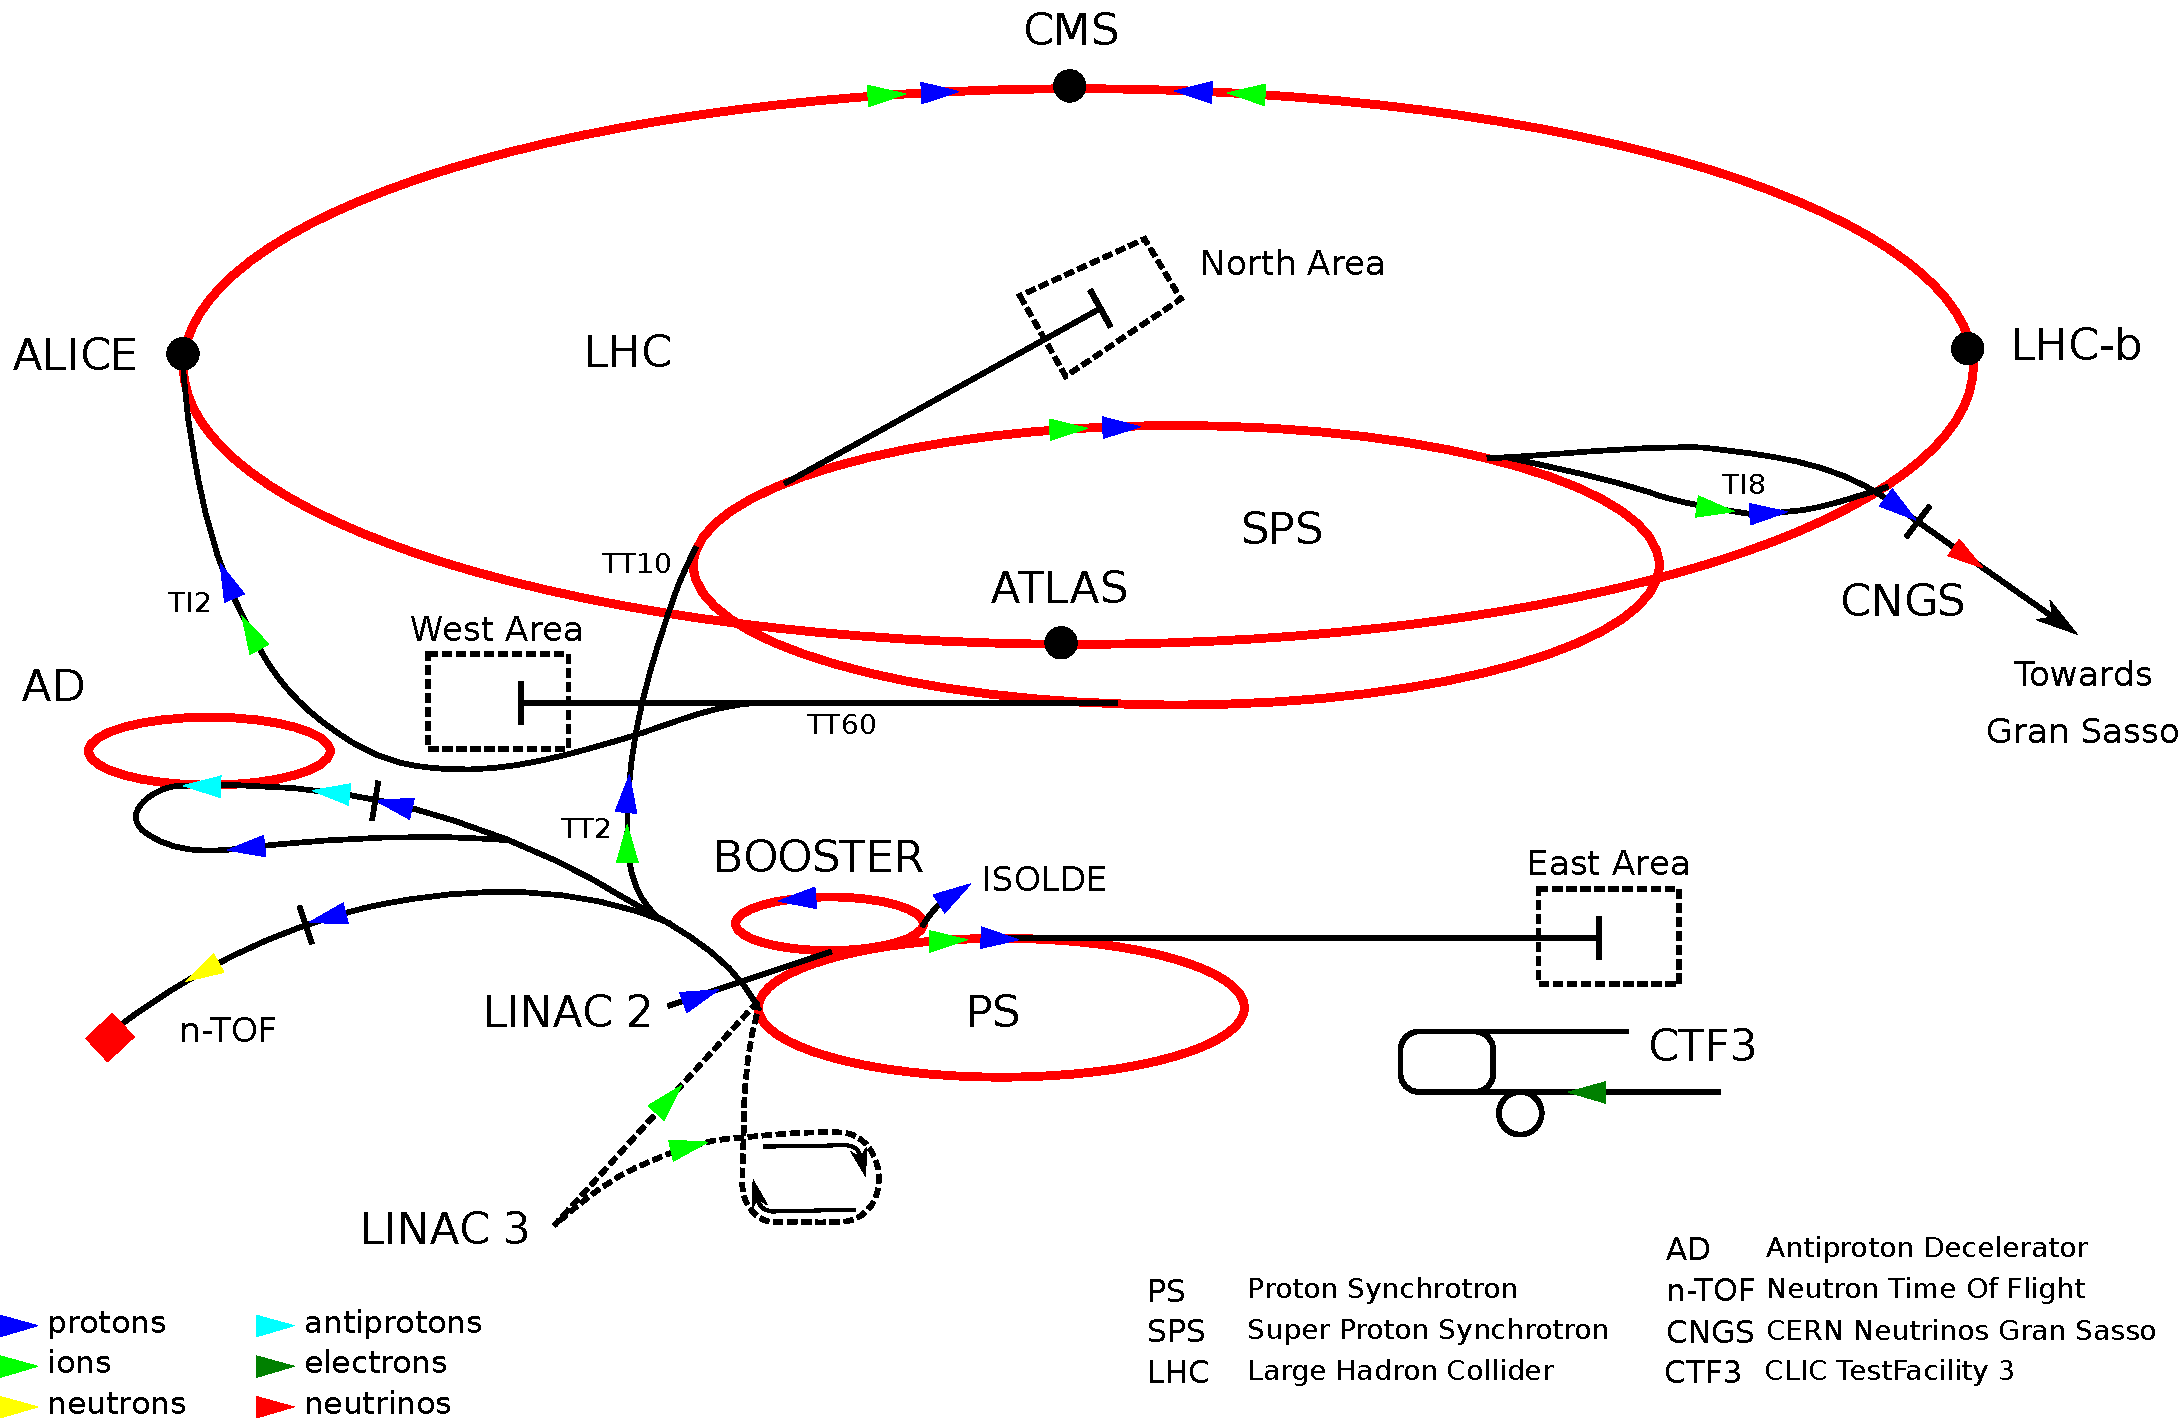
\includegraphics[width=0.92\textwidth]{fig/detector/CERN_accelerator_complex.pdf}
  \vspace{1mm}
  \caption{
CERN's accelerator complex. 
Taken from~\cite{CERN_accelerators}.
  }\label{fig:CERN_complex}
  \vspace{-6mm}
\end{figure*}



%%%%%%%%%%%
%   LHC   %
%%%%%%%%%%%
\section{The Large Hadron Collider}

The Large Hadron Collider (LHC) is the world's largest and most powerful particle collider with a $27\unit{km}$ circumference and a record collision energy of $13.6\TeV$.
It surpasses the Tevatron accelerator at Fermilab in the United States~\cite{Tevatron} ($6.3\unit{km}$, $1.96\TeV$), and LEP ($209\GeV$)~\cite[Section 32]{PDG_2022}.

During the data-taking period of 2015 to 2018, referred to as ``Run 2'', the energy of each proton beam was $6.5\TeV$, which means the center-of-mass energy was $\sqrt{s}=13\TeV$.
The LHC machine is described in more technical detail in Ref.~\cite{LHC}.

% LUMINOSITY
\subsection{Luminosity}\label{sec:lumi}

% FIGURE: luminosity
%!TEX root = ../thesis.tex

% FIGURE: instantaneous luminosity
\begin{figure*}[p]
  \vspace{-6mm}
  \centerline{
    %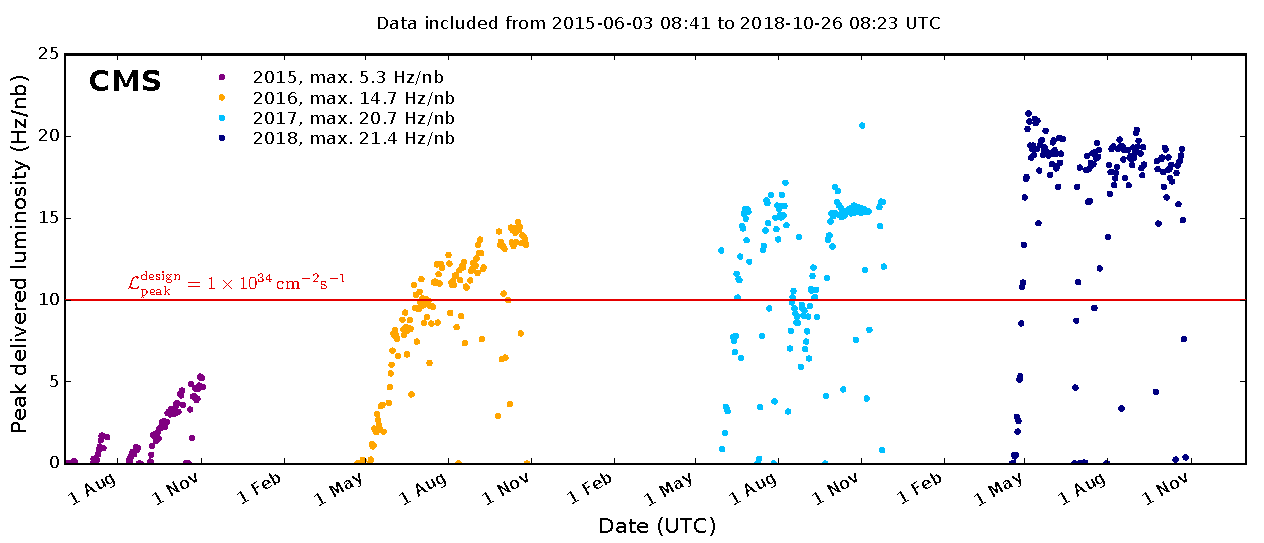
\includegraphics[width=1.04\textwidth,clip,trim={30mm 0mm 16mm 10mm}]{fig/detector/CMS_luminosity_peak_Run2_edit.pdf}
    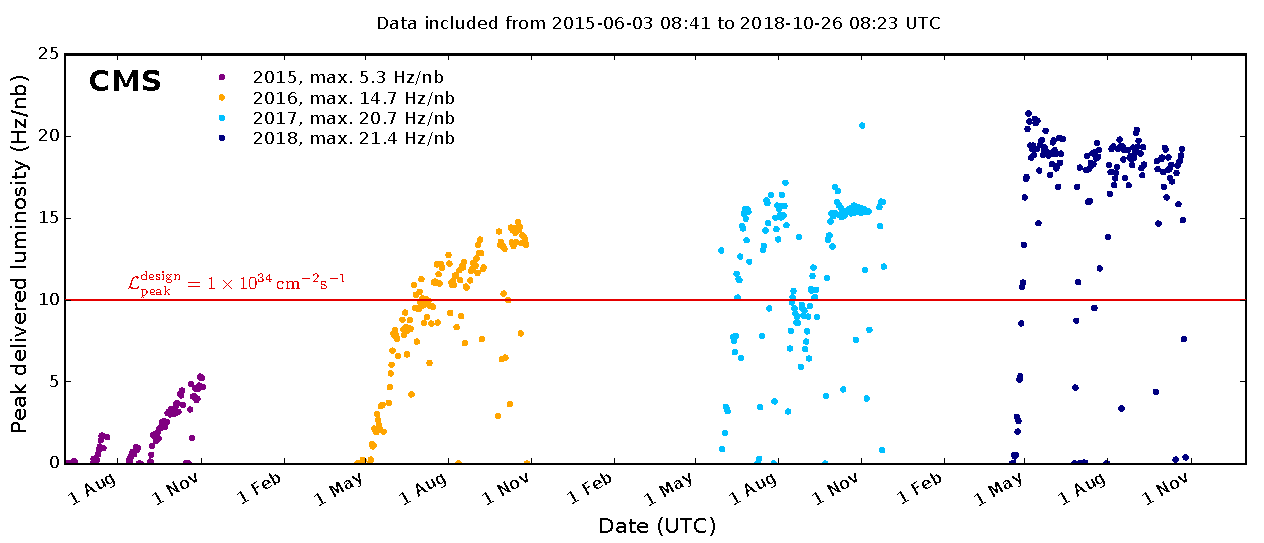
\includegraphics[width=1.04\textwidth]{fig/detector/CMS_luminosity_peak_Run2_edit.pdf}
  }
  \caption{
The instantaneous luminosity \lumi.
The design luminosity is $\lumi^\text{design}_\text{peak}=10^{34}\unit{cm}^{-2}\unit{s}^{-1}$.
Adapted from~\cite{CMS_lumi_TWiki}.
  }\label{fig:CMS_peak_lumi}
  \vspace{-3mm}
\end{figure*}

% FIGURE: integrated luminosity
\begin{figure*}[p]
  \centering
  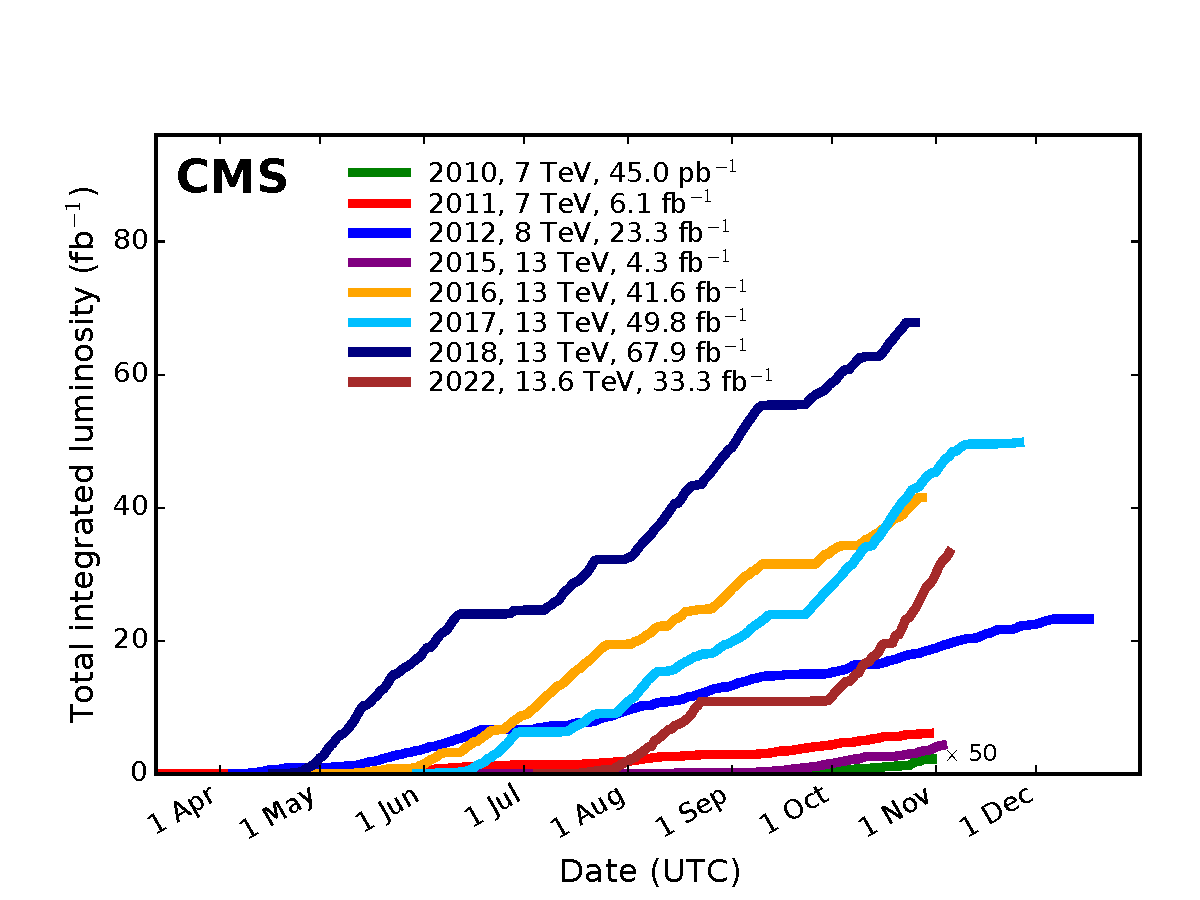
\includegraphics[width=0.57\textwidth,clip,trim={6mm 0mm 6mm 20mm}]{fig/detector/CMS_luminoisty_integrated_Run2.pdf}
  \caption{
Integrated luminosity collected by CMS at $\sqrt{s}=13\TeV$.
Figure taken from~\cite{CMS_lumi_TWiki}.
  }\label{fig:CMS_lumi}
  \vspace{-3mm}
\end{figure*}

% FIGURE: luminosity and pileup
\begin{figure*}[p]
  \centering
  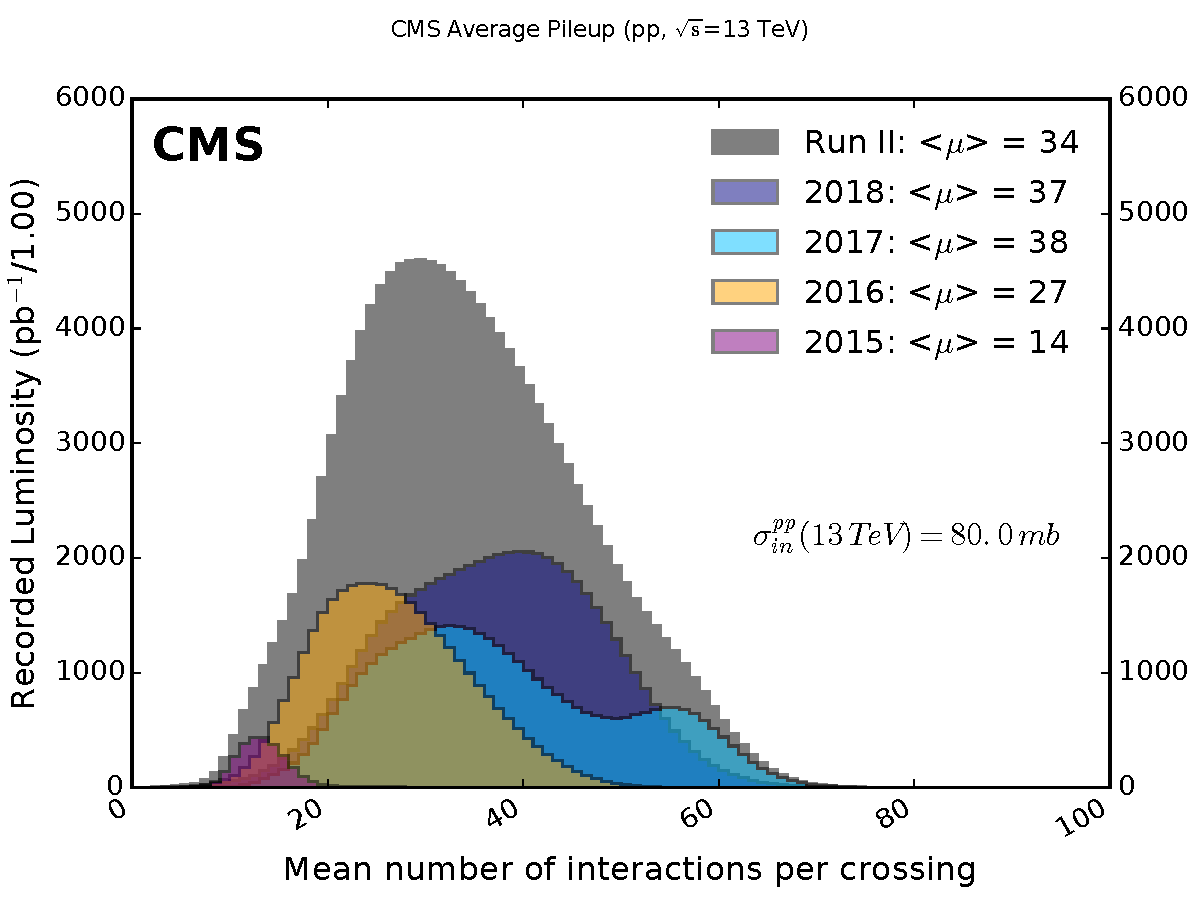
\includegraphics[width=0.58\textwidth,clip,trim={0mm 0mm 0mm 10mm}]{fig/detector/CMS_pileup_Run2.pdf}
  \caption{
Distribution of number of pp interactions, assuming an inelastic cross section of $80\unit{mb}$.
Figure taken from~\cite{CMS_lumi_TWiki}.
  }\label{fig:CMS_pileup}
  \vspace{-4mm}
\end{figure*}


It depends on several beam parameters. The simplified expression is~\cite[p.~533]{PDG_2022}:
\begin{equation}\label{eq:instant_lumi}
  \lumi = \frac{N_1N_2f}{A}.
\end{equation}
The LHC is designed to reach the nominal luminosity of $\lumi=10^{34}\unit{cm}^{-2}\unit{s}^{-1}$.
See \Fig{fig:CMS_peak_lumi}.
Each bunch contains about 110 billion protons~\cite{LHC,LHC_lumi_bunches_Run2}.

% pile up
Figure~\ref{fig:CMS_pileup} shows the distribution of the number of interactions per bunch crossing in all data-taking years of Run 2.

% data
Figure~\ref{fig:CMS_lumi} shows a the data of each data-taking year with \emph{integrated luminosity} $L$, which is
\begin{equation}\label{eq:integrated_lumi}
  L \defeq \int\displaylimits_\text{data taking}\hspace{-4mm}\lumi(t)\text{d}t,
\end{equation}
given in units of inverse area, such as the inverse barn ($\unit{b}^{-1}$).
Between 2016 and 2018, CMS collected about $138\fbinv$ of pp collision data for physics analysis.


%%%%%%%%%%%
%   CMS   %
%%%%%%%%%%%
\section{The CMS detector}
% https://twiki.cern.ch/twiki/bin/viewauth/CMS/Internal/PubDetector

% FIGURE: CMS detector
%!TEX root = ../thesis.tex

% FIGURE: detector
% https://cms-docdb.cern.ch/cgi-bin/PublicDocDB/ShowDocument?docid=12201
\begin{figure*}[b!]
  %\vspace{3mm}
  \centerline{
    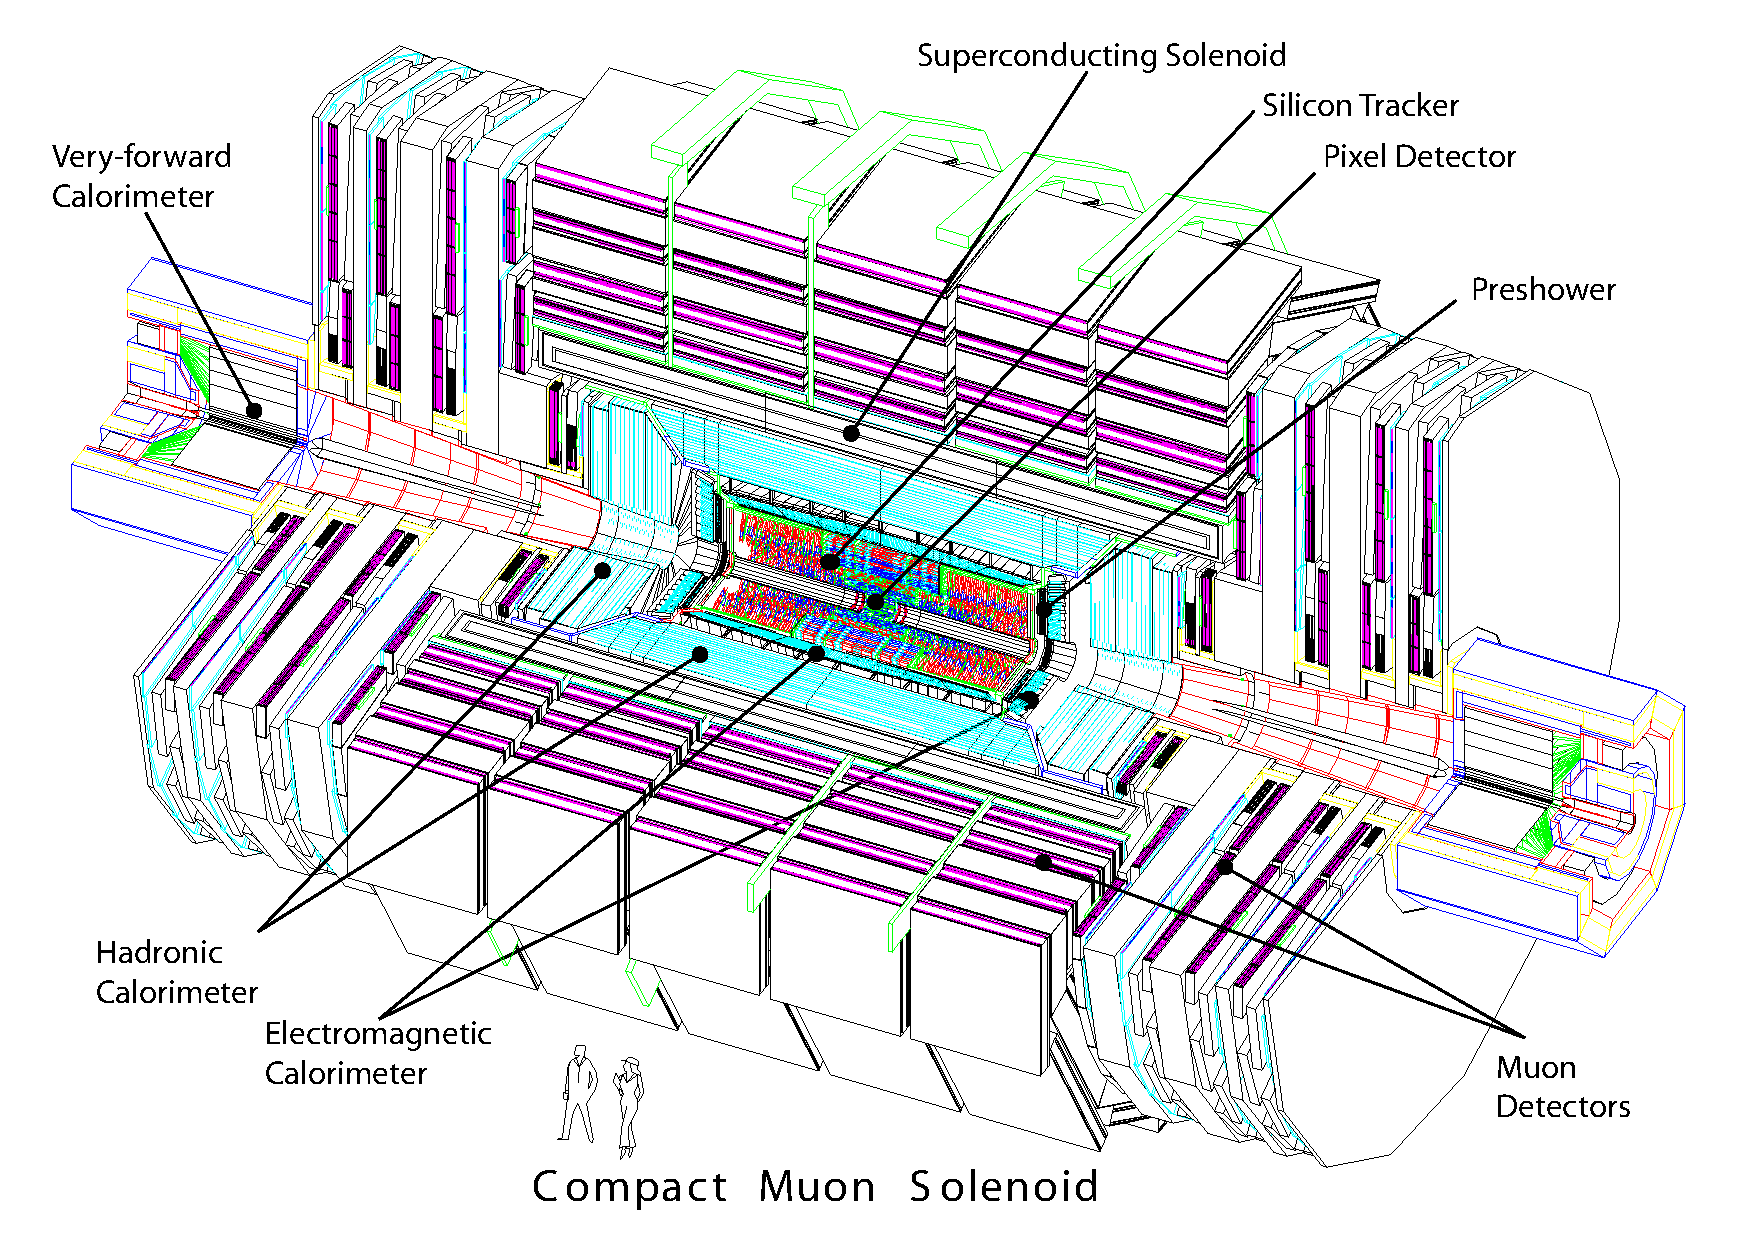
\includegraphics[width=0.92\textwidth,clip,trim={0mm 12.3mm 0mm 0mm}]{fig/detector/CMS_detector_white.pdf}
  }
  \caption{
The CMS detector.
Taken from~\cite{CMS}.
  } \label{fig:CMS}
  %\vspace{-3mm}
\end{figure*}

% FIGURE: coordinate system & eta
\begin{figure*}[b!]
  %\vspace{2mm}
  \centering
  \centerline{
    \raisebox{-0.5\height}{\includegraphics[width=0.7\textwidth,page=4]{fig/detector/CMS_coordinate_system.pdf}}
    \quad
    \raisebox{-0.4\height}{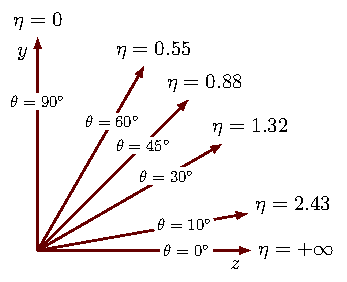
\includegraphics[width=0.32\textwidth]{fig/detector/pseudorapidity_eta_theta.pdf}} 
  }
  %\vspace{-1mm}
  \caption{
\Left: The conventional coordinate system of CMS with momentum vector $\myvec{p}$.
Taken from~\cite{CMS_coordinate_system}.
\Right: Pseudorapidity.
Taken from~\cite{pseudorapidity}.
  } \label{fig:CMS_coordinate_system}
  %\vspace{-3mm}
\end{figure*}

The Compact Muon Solenoid (CMS) detector at one of the interaction points at the LHC.
An illustration is shown in Fig.~\ref{fig:CMS}.
A detailed description can be found in Ref.~\cite{CMS}.

% COORDINATE SYSTEM
\subsection{Coordinate system}
The conventional coordinate system of CMS is defined in Fig.~\ref{fig:CMS_coordinate_system}.

% FIGURE: Subdetectors
%!TEX root = ../thesis.tex

% FIGURE: subdetectors, longitudinal view
\begin{figure*}[p]
  \vspace{-6mm}
  \centering
  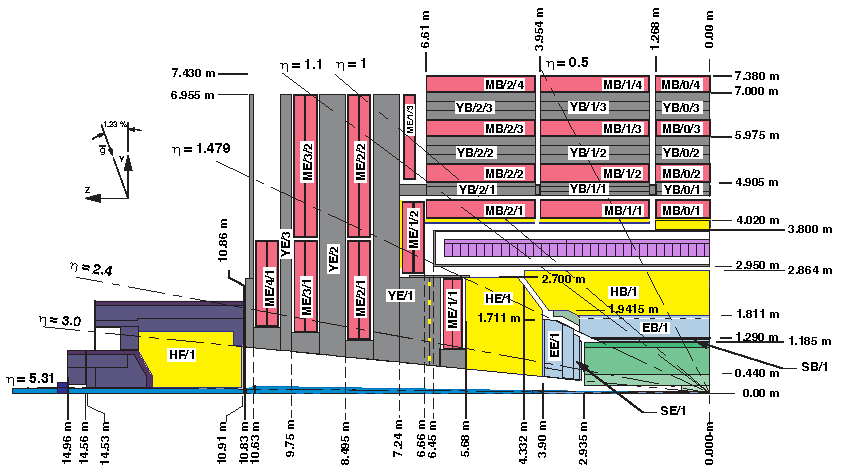
\includegraphics[width=0.92\textwidth]{fig/detector/CMS_detector_longitudinal_edit.pdf}
  %\vspace{-2mm}
  \caption{
Schematic of one quadrant of the CMS detector in the positive $zy$-plane.
Adapted from \cite{CMS_eta}.
  } \label{fig:CMS_eta}
  %\vspace{-2mm}
\end{figure*}

% FIGURE: tracker
\begin{figure*}[p]
  %\vspace{-3mm}
  \centering
  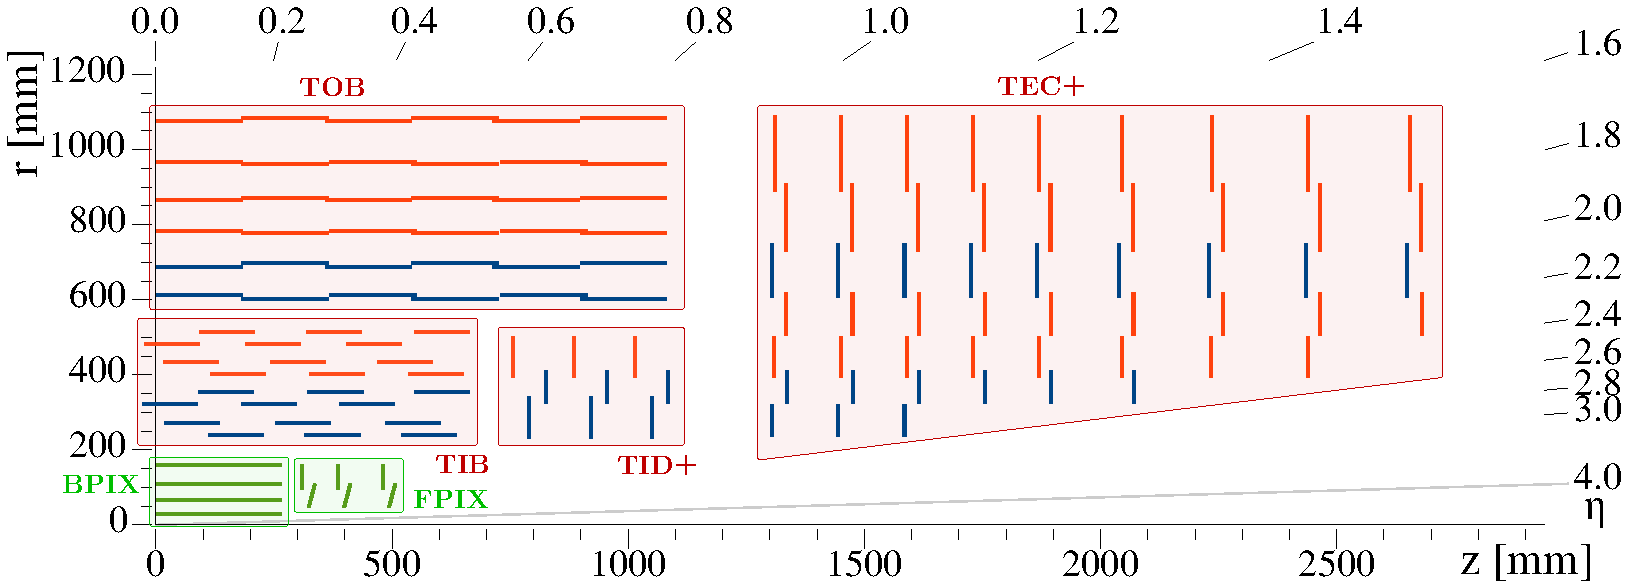
\includegraphics[width=0.8\textwidth]{fig/detector/CMS_tracker_Phase1_edit.pdf}
  %\vspace{-1mm}
  \caption{
Schematic view the CMS tracking system.
Adapted from from~\cite{CMS_tracker_sketch}.
  } \label{fig:CMS_tracker}
  %\vspace{-6mm}
\end{figure*}

% FIGURE: pixel
\begin{figure*}[p]
  %\vspace{-3mm}
  \centering
  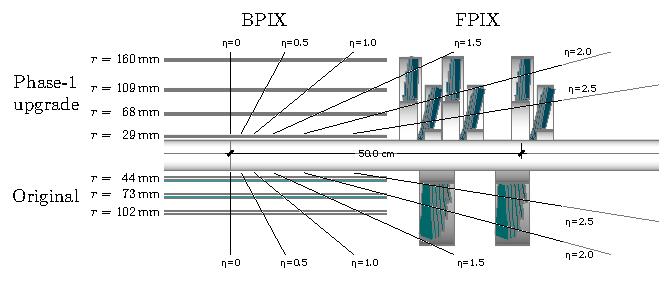
\includegraphics[width=0.86\textwidth]{fig/detector/CMS_pixel_Phase1_edit.pdf}
  \vspace{-2mm}
  \caption{
Layout of the CMS pixel detector.
Adapted from from~\cite{CMS_pixel_Phase1_2021}.
  } \label{fig:CMS_pixel}
  %\vspace{-3mm}
\end{figure*}

% Magnet
\subsection{The solenoid magnet \& flux-return yoke}
The\emph{superconducting solenoid magnet} is a $13\unit{m}$ long cylinder with an inner diameter of $6\unit{m}$.
The yoke~\cite{CMS_yoke}.

% Pixel detector
\subsection{The pixel tracker}
% Description and performance of track and primary-vertex reconstruction with the CMS tracker (2014)
%   https://arxiv.org/pdf/1405.6569.pdf
% The CMS Phase-1 Pixel Detector Upgrade
%   https://cds.cern.ch/record/2748381/files/2012.14304.pdf
% Performance:
%   https://twiki.cern.ch/twiki/bin/view/CMSPublic/TrackingPOGPerformance2017MC
%   https://arxiv.org/pdf/1405.6569.pdf
The inner tracker system has a \emph{silicon pixel tracker} and a \emph{silicon microstrip tracker}. Figure~\ref{fig:CMS_tracker} presents a closer look of the full tracker layout.
The pixel tracker from 2008 up to 2016 was composed of $1440$ sensor modules with a total of $66$ million silicon pixels~\cite{CMS_vertex}.
During the technical shutdown it was upgraded with 1856 modules with 124 million pixels in total~\cite{CMS_pixel_Phase1_2017,CMS_pixel_Phase1_2021}.
Their layouts are compared in \Fig{fig:CMS_pixel}.

% Strip tracker
\subsection{The silicon strip tracker}
% CMS Outer Tracker: Operational Experience, Performance and Lessons Learned
%   https://inspirehep.net/files/0f0440aa2c852ed48ae7cfcf4e6e776a
% Strategies and performance of the CMS silicon tracker alignment during LHC Run 2
%   https://arxiv.org/pdf/2111.08757.pdf (2021)
The silicon strip tracker is larger.
A detailed description of the tracking and vertexing software is given in Ref.~\cite{CMS_vertex}.

% ECAL
\subsection{The electromagnetic calorimeter}
% https://cds.cern.ch/record/349375/files/ECAL_TDR.pdf
The \emph{electromagnetic calorimeter} (ECAL) is built around the tracker.
The energy resolution can be parametrized as a function of energy~\cite{CMS}:
\begin{equation}
  \left(\frac{\sigma_E}{E}\right)^2 = \left(\frac{S}{\sqrt{E}}\right)^2 \oplus \left(\frac{N}{E}\right)^2 \oplus C^2,
\end{equation}
with the stochastic term $S$, the noise $N$, and a constant term $C$.

% HCAL
\subsection{The hadronic calorimeter}
% https://cds.cern.ch/record/2715872?ln=en
The last subdetector inside the solenoid is the \emph{hadron calorimeter} (HCAL).
%The energy resolution can again be parametrized in terms of energy:~\cite{CMS_HCAL}
%\begin{equation}
%  \left(\frac{\sigma}{E}\right)^2 = \left(\frac{S}{\sqrt{E}}\right)^2 \bigoplus B.
%\end{equation}

% Very forward HCAL
The \emph{very forward HCAL} (HF) is positioned around the beamline outside the detector.

% Muon
\subsection{The muon system}
The muon system is outside the solenoid magnet.
The final momentum resolution can be roughly parametrized as follows:
\begin{equation}
  \left(\frac{\sigma_{\pt}}{\pt}\right)^2 = \left(A\cdot\pt\right)^2 \oplus C^2,
\end{equation}
where $A$, and $C$ are constants determined by the hit resolution and multiple scattering, respectively~\cite{CMS_muon_resolution_thesis}. The resolution grows with momentum, because the track becomes more straight, which increases the uncertainty in its curvature.

% TRIGGER
\subsection{The trigger system}\label{sec:trigger}
The collision rate of $40\unit{MHz}$ is higher than is possible to record offline.
The \emph{L1 trigger} has a rate of about $100\unit{kHz}$.
The next level, is the \emph{high-level trigger} (HLT).


